\section{Combinatoria}

\begin{quotation}
	"Serve a contare quanti elementi ci sono in un insieme.
	(risponde alla domanda "Quante sono?")."
\end{quotation}

\mysubsection{Insiemi}
Negli insiemi non conta l'ordine (infatti si usano le "\{\}", se contava l'ordine si usavano le "()") e gli elementi ripetuti. Insieme finito $\{1, \dots, n\}$. Insieme infinito $\{1,\dots\}$.

\definizione{Cardinalità}{Un insieme $A$ ha cardinalità $n$ se contiene esattamente $n$ elementi, o equivalentemente se $\exists$ una corrispondenza biunivoca $A \longleftrightarrow \{1,2,\dots, n\}$.}{d:cardinalita}

La cardinalità si indica $|A|=n$.

\definizione{Insieme finito}{Un insieme $A$ si dice finito se $\exists n \in \mathbb{N}$ t.c. $A$ contiene esattamente $n$ elementi distinti.}{d:insiemefinito}

\osservazione{L'insieme vuoto è l'unico insieme finito di cardinalità 0.}

\definizione{Cardinalità insiemi infiniti}{Due insiemi infiniti hanno la stessa cardinalità se $\exists$ una biezione (Corrispondenza biunivoca) tra di loro.}{d:cardinalitainsiemiinfiniti}

\definizione{Insieme numerabile}{Un insieme $A$ si dice numerabile se ha la stessa cardinalità di $\{1,2,3,\dots\}$.}{d:insiemenumerabile}

In altre parole un insieme è numerabile se i suoi elementi possono essere messi in un a fila infinità.

Insiemi numerabili sono $\mathbb{N}$ (anche se più grande di $\{1,2,3,\dots\}$), $\mathbb{Z}=\{0,1,-1,2,-2,3,\dots\}$, $\mathbb{Q}_{>0}$ dalla dimostrazione classica di Cantor.

Un insieme non numerabile sono delle sequenze infinite di bit 0/1.

\definizione{Insieme Discreto}{Un insieme è discreto se è finito o numerabile.}{d:insiemediscreto}

\mysubsection{Combinatoria di base}
Costruisce schemi "complessi" partendo da schemi semplici riuscendo a controllarne la cardinalità. (si opera solo con insiemi finiti).

\definizione{Prodotto Cartesiano}{Siano $A, B$ insiemi il cui prodotto cartesiano $A \times B$ è l'insieme delle coppie ordinate $(a,b), a \in A, b \in B$.

generalizzando:
\[
A_1 \times A_2 \times \dots \times A_k = \{(a_1, \dots, a_k)\mid a_i\in A_i, \forall i \in 1,\dots, k\}
\]
}{d:prodcart}

\textbf{n-esima potenza cartesiana di n}, ovvero $A \times \dots \times A = A^n$.

\definizione{Sequenza}{Una sequenza (o lista) finita di lunghezza n di elementi di $A$ è un elemento $(a_1,\dots,a_n)$ del prodotto cartesiano $A^n$.}{d:sequenza}

Sono \textbf{successioni} delle sequenze di lunghezza $\infty$, tipo $\{a_1,\dots\}$.

\definizione{Insieme delle parti}{Sia $A$ un insieme, l'insieme delle parti $\mathcal{P}(A)$ è l'insieme i cui elementi sono tutti i sotto insiemi di A, inclusi l'insieme vuoto $\emptyset$ e $A$ stesso. (insieme i cui elementi sono insiemi).}{d:insiemedelleparti}

\teorema{Insieme delle parti}{Sia $A$ un insieme di $|A|=n$, allora $\exists$ una corrispondenza biunivoca tra $\mathcal{P}(A)$ e $\{0,1\}^n$.}{t:insiemedelleparti}

\dimostrazione{t:insiemedelleparti}{Vediamo un caso particolare $A=\{1,2,3\}$

$\{1\}, \{2\}, \{3\}, \{1, 2\}, \{1, 3\}, \{2,3\}, \emptyset, A$

$\updownarrow$

$100=(1,0,0),010,001,110, 101,011,000,111$

Per il caso generale $|A|=n, A=\{a_1,\dots, a_n\}$ procediamo come prima facendo corrispondere ad'un sotto insieme $S\subseteq A$ la sequenza binaria $B$ il uci i-esimo bit è $1\iff a_i\in S$.}

\mysubsection{Principi di base}
\begin{enumerate}
	\item \textbf{Principio di ugualianza:} Siano $A, B$ insiemi qualunque in corrispondenza biunivoca allora questi hanno lo stesso numero di elementi.

	Generalizzazione del Principio di ugualianza: $F:A\to B$ si dice $k:1$ (k a 1) se è surriettiva e a ogni elemento di $B$ corrispondono esattamente $k$ elementi di $A$. In questo caso $|A|=k|B|$. Il principio di ugualianza corrisponde al caso $k=1$.
	\item \textbf{Principio della somma:} Siano $A, B$ insiemi qualunque disgiunti (non hanno elementi in comune), allora $|A\cup B|=|A|+|B|$.

	Ricorda: Si dice Distinti se gli insiemi sono diversi per almeno un elemento.
	\item \textbf{Principio del prodotto:} Siano $A, B$ insiemi qualunque, allora $|A\times B|=|A|\cdot |B|$.
\end{enumerate}

\definizione{Prodotto Condizionato}{Siano $A, B$ insiemi. $C \subseteq A \times B$ è sotto insieme del prodotto cartesiano e si dice prodotto condizionato di tipo $(n,m)$ se sono soddisfatte queste condizioni:
\begin{enumerate}
	\item $\exists n$ elementi di $A$ che compaiono come 1° coefficente in un elemento di $C$.
	\item Fissata la 1° coordinata di un elemento di $C$, $\exists m$ elementi di $B$ che possono essere aggiunti come 2° coordinata.
\end{enumerate}}{d:prodcond}

In altri termini possiamo scegliere la 1° coordinata in n modi e fissata questa scelta possiamo scegliere la 2° in m modi.

Se per tutti i primi n coefficenti si hanno m secondi coefficienti si ha il prodotto condizionato, altrimenti no.

Una coordinata può non essere scelta.

\definizione{Disposizioni}{Sia $A=\{1,\dots,n\}$ una disposizione di lungheza $k$ in $A$, è una sequenza $(a_1,\dots,a_k)$ di $A$ t.c. $a_i\ne a_j, \forall i \ne j$.}{d:disposizione}

\proposizione{Fattoriale Discendente}{Le disposizioni di lunghezza $k$ in $\{1,\dots,n\}$ sono \[\underbrace{n(n-1)\cdots(n-k+1)}_{k}=(n)_k\]}{prop:fattorialediscreto}

\dimostrazione{prop:fattorialediscreto}{Abbiamo $n$ scelte per la prima coordinata. Fissata la prima coordinata ho $n-1$ scelte per la seconda coordinata. Fissate le prime due coordinate ho $n-2$ scelte per la terza coordinata, e cosi via. Abbiamo quindi un prodotto condizonato di tipo $(n,n-1,\dots,n-k+1)$.}

\definizione{Permutazioni}{Una permutazione di lunghezza $n$ è una disposizione di lunghezza $n$ in $\{1,\dots,n\}$.}{d:permutazione}

Conseguenza: Dal Fattoriale Discreto, il numero di permutazioni di lunghezza $n$ è $(n)_n=1\cdot2\dots n=n!$.

\definizione{Combinazioni}{Sia $A=\{1,\dots,n\}$, una combinazione è un sotto insieme di $A$ con $a$ elementi. (l'ordine non importa).}{d:combinazione}

\proposizione{Numero Combinazioni}{Siano $a,b,n$ con $a+b=n$, allora questi 3 insiemi sono in biezione tra loro.
\begin{enumerate}
	\item Sotto insieme di $\{1,\dots,n\}$ con $a$ elementi.
	\item Sotto insieme di $\{1,\dots,n\}$ con $n$ elementi.
	\item Sequenza binarie lunghezza $n$ con $a$ volte 1 e $b$ volte 0.
\end{enumerate}
Questi insiemi hanno esattamente $\frac{(n)_a}{a!}=\frac{(n)_b}{b!}=\frac{n!}{a!b!}$ elementi.}{prop:combinazioni}

Questo numero $\frac{(n)_a}{a!}=\binom{n}{a}=\binom{n}{a,b}$.

Coefficente binomiale:
\[
(x+y)^n=\sum_{a=0}^n\binom{n}{a}x^ay^{n-a}=\sum_{a,b\mid a+b=n}\binom{n}{a,b}x^ay^b
\]

\dimostrazione{prop:combinazioni}{$(Parte1)$ La corrispondenza tra 1 e 3 la si dimostra con il seguene esempio: $n=5, a=3$
\[
\begin{aligned}
	\{1,2,3\} \leftrightarrow 11100\\
	\{1,2,4\} \leftrightarrow 11010\\
	\{1,2,5\} \leftrightarrow 11001\\
	\{1,3,4\} \leftrightarrow 10110\\
\end{aligned}
\]
Tutte le sequenze hanno 3 "1" e 2 "0".

Poi 1 e 2 sono in biezione data dal completamento.

$(Parte2)$ Pensiamo di avere una funzione fatta cosi: Nel dominio abbiamo le disposizioni di lunghezza $a$ in $\{1,\dots,n\}$ e nel codominio abbiamo i sotto insiemi di $\{1,\dots,n\}$ con $a$ elementi. Per esempio:
\[
\begin{aligned}
	(2,5,1) \mapsto \{1,2,5\}\\
	(3,5,4) \mapsto \{3,4,5\}\\
	(3,4,5) \mapsto \{3,4,5\}\\
\end{aligned}
\]
Non è in biezione perchè non è ignettiva. (Nel caso generale abbiamo una funzione $a!:1$).

Quindi le disposizioni sono $A!$ volte i sotto insiemi e quindi i sotto insiemi con $a$ elementi sono $\frac{(n)_a}{a!}=\frac{n(n-1)\dots(b+1)}{a!}=\frac{n(n-1)\dots3\cdot2\cdot1}{a!b!}=\frac{n!}{a!b!}$.}

\definizione{Combinazione di 1\dots n}{Una combinazione di lunghezza $a$ in $\{1,\dots,n\}$ è un sotto insieme di $\{1,\dots,n\}$ con $a$ elementi.}{d:combsottoins}

\definizione{Combinazione tipo (a,b)}{Una combinazione di tipo $(a,b)$ con $(a+b=n)$ è una coppia ordinata $(A,B)$ di sotto insiemi di $\{1,\dots,n\}$ con $|A|=a,|B|=b,A\cup B=\{1,\dots,n\}$.}{d:combtipo2}

\definizione{Combinazione tipo (a,b,c)}{Una combinazione di tipo $(a,b,c)$ con $(a+b+c=n)$ è una terna ordinata $(A,B,C)$ di sotto insiemi di $\{1,\dots,n\}$ con $|A|=a,|B|=b, |C|=c,A\cup B \cup C=\{1,\dots,n\}$.}{d:combtipo3}

\definizione{Anagramma}{Sequenza ordinate di numeri $\{1,\dots,n\}$ con $n=a+b+\dots$ binarie, ternarie, quaternarie, ecc di tipo $(a,b,c,\dots)$ in biezione con le sequenze in cui compare $a$ volte "1", $b$ volte "2", $c$ volte "3", ecc.}{d:anagramma}

Esempio di riferimento (terna):
\[
\begin{aligned}
	(\{1,2\}, \{3\}, \{4\}) \leftrightarrow (1,1,2,3)\\
	(\{1,2\}, \{4\}, \{3\}) \leftrightarrow (1,1,2,3)\\
	(\{1,3\}, \{2\}, \{4\}) \leftrightarrow (1,2,1,3)\\
	(\{2,4\}, \{1\}, \{3\}) \leftrightarrow (2,1,3,1)\\
\end{aligned}
\]

\proposizione{Binomio Combinazioni tipo (a,b,c)}{Le combinazioni di tipo $(a,b,c)$ con $(a+b+c=n)$ sono $\binom{n}{a,b,c}=\frac{n!}{a!b!c!}$.}{prop:tipo3binomio}

\dimostrazione{prop:tipo3binomio}{Posso scegliere $A$ in $\binom{n}{a}$ modi. Fissato $A$ posso sciegliere $B$ in $\binom{n-a}{b}$ modi. $C$ è univocamente determinato da $A,B$.

Il numero di combinazioni di tipo $(a,b,c)$ è $\binom{n}{a}\cdot\binom{n-a}{b}=\frac{n!}{a!(n-a)!}\cdot\frac{(n-a)!}{b!(n-a-b)!}=\frac{n!}{a!b!c!}$.}

\osservazione{$\binom{n}{a,b,c}=\binom{n}{b,c,a}$=\dots, in particolare con due indici abbiamo $\binom{n}{a}=\binom{n}{b}$ se $(a+b=n)$.}

\proposizione{Somma binomi}{$\binom{n}{a,b}=\binom{n-1}{a-1,b}+\binom{n-1}{a,b-1}$ che è uguale a $\binom{n}{a}=\binom{n-1}{a-1}+\binom{n-1}{a}$.

Più in generale $\binom{n}{a,b,c}=\binom{n-1}{a-1,b,c}+\binom{n-1}{a,b-1,c}+\binom{n-1}{a,b,c-1}$.}{prop:sommabinomi}

\dimostrazione{prop:sommabinomi}{Le combinazioni di tipo $(a,b,c)$ sono in biezione con le combinazioni di tipo:
\begin{itemize}
	\item $\{(A,B,C)\mid n \in A\}$ sono $\binom{n-1}{a-1,b,c}$.
	\item $\{(A,B,C)\mid n \in B\}$ sono $\binom{n-1}{a,b-1,c}$.
	\item $\{(A,B,C)\mid n \in C\}$ sono $\binom{n-1}{a,b,c-1}$.
\end{itemize}}

\mysubsection{Cammino Reticolare}
\begin{center}
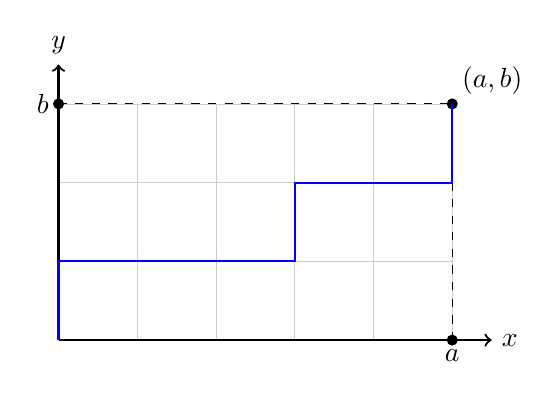
\begin{tikzpicture}[scale=1]
	% Griglia di sfondo
	\draw[step=1cm,gray!40,very thin] (0,0) grid (5,3);

	% Assi
	\draw[->,thick] (0,0) -- (5.5,0) node[right] {$x$};
	\draw[->,thick] (0,0) -- (0,3.5) node[above] {$y$};

	% Punti (0,b), (a,0), (a,b)
	\fill (0,3) circle (2pt) node[left] {$b$};
	\fill (5,0) circle (2pt) node[below] {$a$};
	\fill (5,3) circle (2pt) node[above right] {$(a,b)$};

	% Linee tratteggiate perpendicolari
	\draw[dashed] (5,0) -- (5,3);
	\draw[dashed] (0,3) -- (5,3);

	% Curva a gradini (simile a quella verde nell’immagine)
	\draw[blue,thick]
	(0,0) -- (0,1) -- (1,1) -- (2,1) -- (3,1) -- (3,2) -- (4,2) -- (5,2) -- (5,3);

\end{tikzpicture}
\end{center}

Il cammino reticolare nel piano cartesiano è il percorso che congiunge l'orgine degli assi a un punto (a,b) tramite \textit{passi} verticali o orrizontali di 1.

Ottima interpretazione grafica di una combinazione di tipo (a,b).
Quanti sono i cammini reticolari da (0,0) a (a,b)?

Possiamo codificare i passi inverticali con "1" e i passi orrizontali con "0". Cosi i cammini grafici diventano sequenze binarie. La lunghezza di tali sequenze è $a+b$, con $a$ volte "0" e $b$ volte "1". Abbiamo ottenuto un anagramma di tipo (a,b).

Osserviamo che abbiamo una biezione tra cammini e anagrammi e i cammini sono quindi $\binom{a+b}{a,b}$.

\mysubsection{Numeri di Fibonacci}
Conta i sotto insiemi di $\{1,\dots,n\}$ che non hanno 2 numeri consecutivi.

\[F_n=\sum_{k=0}^n\binom{n-k+1}{k}\]

\textbf{Ragionamento}, Definiamo:

\begin{itemize}
	\item $F_n$ come il numero di sotto insiemi possibili di $\{1,\dots,n\}$.
	\item $F_{n,k}$ il numero di sotto insiemi di $\{1,\dots,n\}$ di $k$ elementi che non hanno due elementi consecutivi.
\end{itemize}

Arriviamo alla formula con un esempio, $F_{8,3}$. Vediamo questi insiemi come sequenze di lunghezza 8 con 3 "1" non consecutivi (astrazione simile Camminio Reticolare). Devo riuscire ad'usare il principio d'equivalenza con un insieme di cui so la cardinalità. Sò che dopo il primo e secondo "1" c'è sempre uno "0", quindi cancello questo "0" cosi ho sequenze da 6.
Ora "1" possono essere consecutivi ma posso tornare univocamente alla precedente rappresentazione, quindi è biunivoco.
Deduciamo che $F_{8,3}=\binom{6}{3}=20$.

In generale $F_{n,k}$ sono le sequenze di lunghezza $n$ con $k$ volte "1", non consecutivi. Cancellando gli "0" che seguono i primi $k-1$ "1" otteniamo una sequenza binaria lunga $n-k+1$, con $k$ "1".

Tali sequenze sono $F_{n,k}=\binom{n-k+1}{k}$ e quindi $F_n=\sum_{k=0}^n\binom{n-k+1}{k}$.
A $n$ non ci arrivo perchè il coefficente binomiale da 0 quando $k>n-k+1$.